\documentclass[11pt]{article}
\usepackage{geometry, titlesec}
\usepackage[parfill]{parskip}
\usepackage[italicdiff]{physics}
\usepackage{amsfonts, amsthm}
\usepackage[cm]{fullpage}
\usepackage{fancyhdr}
\usepackage{enumitem}
\usepackage{xcolor, soul}
\usepackage{graphicx}
\usepackage[export]{adjustbox}
\usepackage{siunitx}
%\allowdisplaybreaks

\renewcommand{\thesubsection}{\thesection.\alph{subsection}}
\setenumerate[1]{label={(\alph*)}}

\makeatletter
\renewcommand*\env@cases[1][1.2]{%
  \let\@ifnextchar\new@ifnextchar
  \left\lbrace
  \def\arraystretch{#1}%
  \array{@{}l@{\quad}l@{}}%
}
\makeatother
 
\renewcommand{\footrulewidth}{.2pt}
%\setlist[enumerate]{leftmargin=*}
\pagestyle{fancy}
\fancyhf{}
\lhead{Physics 132-B}
\chead{\textbf{Discussion 8 Solutions}}
\rhead{A--De Discussion}
\setlength{\headheight}{11pt}
\setlength{\headsep}{11pt}
\setlength{\footskip}{24pt}
\lfoot{\today}
\rfoot{\thepage}

\titleformat{\subsection}[runin]{\normalfont\large\bfseries}{\thesubsection}{1em}{}
\newcommand{\refeq}[1]{(\ref{#1})}

\newcommand{\beq}{\begin{equation*}}
\newcommand{\eeq}{\end{equation*}}

\newcommand{\beqn}{\begin{equation}}
\newcommand{\eeqn}{\end{equation}}

\newcommand{\blg}{\begin{align*}}
\newcommand{\elg}{\end{align*}}


\newenvironment{statement}
{
    \color{gray}
    \ignorespaces
}
{
%    \smallskip
}

\newenvironment{problem}
{
    \color{darkgray}
    \ignorespaces
}

\newenvironment{solution}
{
    \paragraph{Solution.}
    \ignorespaces
}
{
    \bigskip
}

\newcommand{\qimplies}{\quad \implies \quad}
\newcommand{\qto}{\quad \to \quad}

\renewcommand{\medskip}{\vspace{8pt}}


\begin{document}
	

\newcommand{\vA}{\vb{A}}
\newcommand{\vB}{\vb{B}}
\newcommand{\vE}{\vb{E}}
\newcommand{\vF}{\vb{F}}
\newcommand{\vl}{\vb{l}}
\newcommand{\PhiB}{\Phi_B}
\newcommand{\cE}{\mathcal{E}}
\newcommand{\muo}{\mu_0}
\newcommand{\enc}{\text{enc}}
\newcommand{\Ienc}{I_\enc}

\paragraph{Question 29.1}
\begin{problem}
	A sheet of copper is placed between the poles of an electromagnet with the magnetic field perpendicular to the sheet.  When the sheet is pulled out, a considerable force is required, and the force required increases with speed.  Explain.  Is a force required also when the sheet is inserted between the poles?  Explain.
\end{problem}

\begin{solution}
	When the sheet is between the poles, there is a magnetic flux $\PhiB$ through it, given by
	\beqn \tag{27.6}
		\PhiB = \int \vB \vdot \dd{\vA},
	\eeqn
	where $\vB$ is the magnetic field, and $\vA$ has magnitude equal to the area of the sheet in the field and direction perpendicular to the sheet's suface.
	
	When the sheet is pulled out, its area in the $\vB$ field, $A$, decreases.  This means that $\PhiB$ through the sheet decreases, and this decrease is proportional to the speed $v$ at which we pull the sheet.  Say the sheet is a square of side length $L$.  Then $\dv*{A}{t} = L v$, and so
	\beq \tag{*}
		\dv{\PhiB}{t} \propto \dv{A}{t} \propto -v,
	\eeq
	where the sign is negative because we are pulling the sheet \emph{out}.  From Faraday's law of induction,
	\beq \tag{29.3}
		\cE = -\dv{\PhiB}{t},
	\eeq
	an emf $\cE$ will be induced in the sheet.
	
	Since we are working with a sheet (as opposed to a wire), the emf creates eddy currents $I$ in the sheet.  By Lenz's law, the direction of these currents will oppose the decrease in magnetic flux.  There is a magnetic force exerted on these currents, from 
	\beqn \tag{27.19}
		\vF = I \vl \cross \vB.
	\eeqn
	In summary, $\vF \propto I$ from Eq.~(27.19), $I \propto -\dv*{\PhiB}{t}$ from Eq.~(29.3), and $\dv*{\PhiB}{t} \propto -v$ from (*).  So we see that $\vF \propto v$, as expected.
	
	When the sheet is inserted between the poles, the only change is that $A$ is \emph{increasing} with time.  So $\dv*{\PhiB}{t} \propto v$, and then $\vF \propto -v$.  This means that the force is in the opposite direction of what it was before, but we are also moving the sheet in the opposite direction as before.  So the force still resists the motion of the sheet.
\end{solution}


%\clearpage
\paragraph{Question 29.3}
\begin{problem}
	Two circular loops lie side by side in the same plane.  One is connected to a source that supplies an increasing current; the other is a simple closed ring.  Is the induced current in the ring in the same direction as the current in the loop connected to the source, or opposite?  What if the current in the first loop is decreasing?  Explain.
\end{problem}

\begin{solution}
	\vspace{2in}
	
	Say current is flowing clockwise through the loop connected to the source, as shown.  Using the right hand rule, the magnetic field created by this current will be pointing \emph{up} through the center of the ring.
	
	When the current in the loop is increasing, the magnetic flux $\PhiB$ through the area of the ring is increasing.  By Lenz's law, a current will be induced in the ring whose direction opposes this increase in $\PhiB$.  So the current through the loop will be in the direction to create a magnetic field that points \emph{down} through the center of the ring.  Using the right-hand rule, this means the current flows clockwise, which is the same direction as the currents in the loop.
	
	When the current in the loop is decreasing, so is $\PhiB$.  Lenz's law tells us that the induced current will now slow in such a way to make up for this decrease; that is, to create a magnetic field that points \emph{up} through the center of the ring.  For our example, this is counterclockwise by the right-hand rule.  So the currents are now in opposite directions.
\end{solution}



\paragraph{Question 29.13}
\begin{problem}
	A metal ring is oriented with the plane of its area perpendicular to a spatially uniform magnetic field that increases at a steady rate.  If the radius of the ring is doubled,
	\begin{enumerate}
		\item by what factor does the emf induced in the ring change, and
		\item by what factor does the electric field induced in the ring change?
	\end{enumerate}
\end{problem}

\begin{solution}
	Let $r$ be the initial radius of the ring.
	\begin{enumerate}
		\item As in Question~29.1, the emf $\cE$ induced in the ring is given by Faraday's law,
			\beq \tag{29.3}
				\cE = -\dv{\PhiB}{t},
			\eeq
			where the magnetic flux $\PhiB$ is given by
			\beqn \tag{27.6}
				\PhiB = \int \vB \vdot \dd{\vA}.
			\eeqn
			In this problem, the time dependence in $\PhiB$ is due to $\vB$ only.
			
			If the radius of the ring is doubled, $r \to 2r$, then the area of the ring increases by a factor of four:
			\beq
				A = \pi r^2
				\qto
				\pi (2r)^2 = 4 \pi r^2 = 4A.
			\eeq
			This means the magnetic flux through the ring increases by a factor of four, and so does its time derivative:
			\beq
				A \to 4A
				\qimplies
				\PhiB \to 4\PhiB
				\qimplies
				\dv{\PhiB}{t} \to 4 \dv{\PhiB}{t}.
			\eeq
			By Eq.~(29.3), we have $\cE \to 4 \cE$.  So the emf induced in the ring increases by a factor of four.
			
		\item The statement of Faraday's law relating to the electric field $\vE$ is
			\beqn \tag{29.10}
				\oint \vE \vdot \dd{\vl} = -\dv{\PhiB}{t},
			\eeqn
			where $\vE$ is the electric field around a path traced out by $\vl$.  For this problem, we are taking a path integral around the circumference of the ring.  This means
			\beq
				\oint \vE \vdot \dd{\vl} = (2\pi r) E
				\qimplies
				E = \frac{1}{2\pi r} \abs{\dv{\PhiB}{t}}.
			\eeq

			If the radius of the ring is doubled,
			\beq
				2\pi r \to 2\pi (2r) = 4\pi r,
			\eeq
			and we know from (a) that $\dv*{\PhiB}{t} \to 4 \dv*{\PhiB}{t}$.  Putting these together,
			\beq
				E = \frac{1}{2\pi r} \abs{\dv{\PhiB}{t}}
				\qto
				\frac{1}{4\pi r} \abs{4 \dv{\PhiB}{t}} = \frac{1}{\pi r} \abs{\dv{\PhiB}{t}} = 2E,
			\eeq
			so the electric field induced in the ring increases by a factor of two.
	\end{enumerate}
\end{solution}



\newcommand{\intab}{\int_a^b}

\begin{minipage}[l]{0.65\textwidth}
\paragraph{Problem 29.7}
\begin{problem}
	The current in the long, straight wire shown in \textbf{Fig.~E29.7} is upward and is increasing steadily at a rate $\dv*{i}{t}$. \medskip
	\begin{enumerate}
		\item At an instant when the current is $i$, what are the magnitude and direction of the field $\vB$ at a distance $r$ to the right of the wire?  (Use Ampere's law to find the magnitude.) \medskip
		\item What is the flux $\dd{\PhiB}$ through the narrow, shaded strip? \medskip
		\item What is the total flux through the loop? \medskip
		\item What is the induced emf in the loop? \medskip
		\item Evaluate the numerical value of the induced emf if $a = \SI{12.0}{\cm}$, $b = \SI{36.0}{\cm}$, $L = \SI{24.0}{\cm}$, and $\dv*{i}{t} = \SI{9.60}{\ampere\per\second}$.
	\end{enumerate}
\end{problem}
\end{minipage}%
\hspace{0.05\textwidth}%
\begin{minipage}[r]{0.30\textwidth}
\center 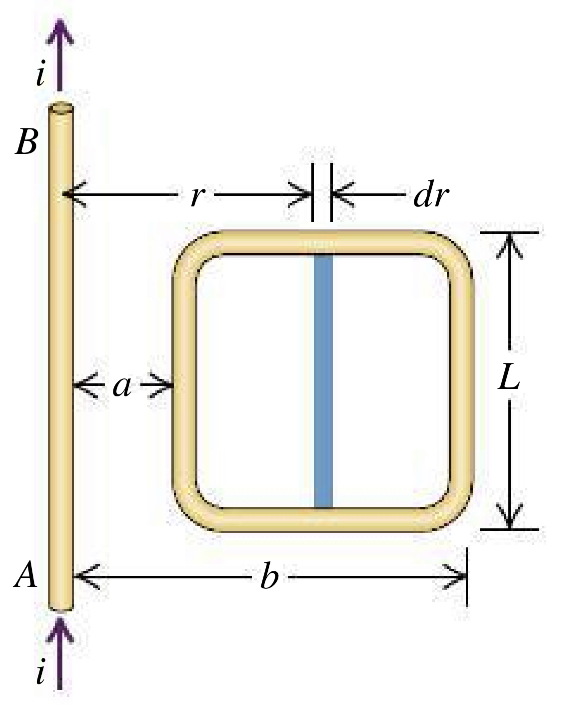
\includegraphics[width=\textwidth]{P29-7.jpeg}
\center \textbf{Figure E29.7}
\end{minipage}

\begin{solution}
	\begin{enumerate}
		\item Ampere's law is
			\beqn \tag{28.20}
				\oint \vB \vdot \dd{\vl} = \muo \Ienc.
			\eeqn
			Let's choose our Amperian loop to be a circle of radius $r$ with the wire pointing through its center:
			
			\vspace{2in}
			
			Then the path integral reduces to
			\beq
				\oint \vB \vdot \dd{\vl} = (2\pi r) B,
			\eeq
			which gives us
			\beq
				B = \frac{\muo \Ienc}{2\pi r}.
			\eeq
			For the direction, the right-hand rule tells us $\vB$ points counterclockwise around the wire.  To the right of the wire, $\vB$ is pointing into the page.  So
			\beq
				\vB = \frac{\muo i}{2\pi r}, \quad \text{into the page.}
			\eeq
			
		\item The magnetic flux is given by
			\beqn \tag{27.6}
				\PhiB = \int \vB \vdot \dd{\vA}.
			\eeqn
			The narrow, shaded strip has area
			\beq
				\dd{A} = L \dd{r},
			\eeq
			and its normal is perpendicular to the page, which is parallel to $\vB$.  This means
			\beq
				\dd{\PhiB} = B \dd{A} = \frac{\muo i L}{2\pi r} \dd{r}.
			\eeq
			
		\item In order to find the total flux $\PhiB$ through the loop, we need to integrate $\dd{\PhiB}$ over $r$.  The width of the loop is $b - a$, so we will integrate from $r = a$ to $r = b$:
			\beq
				\PhiB = \intab \dd{\PhiB}
				= \intab \frac{\muo i L}{2\pi r} \dd{r}
				= \frac{\muo i L}{2\pi} \intab \frac{\dd{r}}{r}
				= \frac{\muo i L}{2\pi} \bigg[ \ln r \bigg]_a^b
				= \frac{\muo i L}{2\pi} (\ln b - \ln a)
				= \frac{\muo i L}{2\pi} \ln(\frac{b}{a}).
			\eeq
			
		\item The induced emf in the loop can be found by Faraday's law,
			\beq \tag{29.3}
				\cE = -\dv{\PhiB}{t}.
			\eeq
			Here, we know that the current is increasing with rate $\dv*{i}{t}$.  Nothing else about the flux is changing, so
			\beq
				\abs{\cE} = \dv{\PhiB}{t} = \frac{\muo L}{2\pi} \ln(\frac{b}{a}) \dv{i}{t}.
			\eeq
			
		\item Plugging in the given values, and $\muo$ from the back cover of the textbook,
			\begin{align*}
				\abs{\cE} &= \frac{(\SI{1.257e-6}{\weber\per\ampere\per\meter}) (\SI{0.240}{\meter})}{2\pi} \ln(\frac{\SI{0.360}{\meter}}{\SI{0.120}{\meter}}) (\SI{9.60}{\ampere\per\second}) \\
				&= \frac{(\num{1.257e-6}) (0.24) (9.6) (\ln 3)}{2 \pi} \,\si{\weber\per\second} \\
				&= \frac{(\num{1.257e-6}) (0.24) (9.6) (1.099)}{2 \pi} \,\si{\volt} \\
				&= \SI{5.07e-7}{\volt}
				= \SI{507}{\nano\volt},
			\end{align*}
			where we have used $\SI{1}{\weber} = \SI{1}{\volt\second}$.
			
			Notice that the induced emf is very, very tiny, even though the current is increasing rapidly!  This demonstrates how small of an effect induction is.
	\end{enumerate}
\end{solution}

\end{document}